% OCR draft from PDF pages 83-113. Needs cleanup and verification.
\chapter{Model Development and Testing}
\label{chap:model-development-testing}

\section{The Modeling and Analysis Process}
\label{sec:modeling-analysis-process}

This and the following chapter discuss the steps involved in developing and
using a simulation model. The key step in this process is that of abstracting
 a system design into a model design. No amount of discussion of this task can
take the place of experience, and even the experienced modeler finds new
challenges in each new system. The sooner you translate your interest in
simulation into experience, the better! It is useful to spend some time
building simulation models of queueing systems with known analytic solutions
 to become familiar with smpl, to develop simulation programming skills, and
to gain experience with the output analysis methods discussed in the next
chapter. To develop skills in abstracting from system design to model,
though, requires working with an actual system. It is best to begin with an
existing system with which you're familiar, and for which data can be obtained
for workload characterization and model validation. Start with a simple model:
if possible, select a modest subsystem that can be isolated from the rest of
the system. Picking a modeling subject in advance of reading this chapter will
help establish a context for the discussion which follows.

The modeling and analysis process is outlined in Figure 3.1. (The nice linear
flow shown in this figure rarely happens in practice; we'll usually go through
several iterations of parts of this process.) The process can be divided into
three phases: development, testing, and analysis. This chapter is concerned
with the development and testing phases.

The first step in development is describing system operation from a
performance viewpoint. This description then is abstracted, in accordance
with the objectives of the analysis, into a model description. This specifies
the facilities to be represented in the model and their interconnection, the
work to be represented and its attributes, and the operations involved in
accomplishing this work. The level of the detail of the model determines the
data to be collected. Next, the appropriate analysis method is chosen, and a
model implementation is developed. We'll assume this takes the form of a
simulation program; alternatively, it could involve translating the model
design and data to input parameters for a queueing network analysis package.

The testing phase comprises three steps: debugging, verification, and
validation. All too often, the simulation program is considered to be
debugged when it runs to completion without errors and produces
``reasonable'' results: single-server facility utilizations are between 0 and 1,
and so on. Verification insures that the simulation program is indeed an
implementation of the model. Validation insures that the model is a
reasonable representation of the real system.

\begin{figure}[ht]
\centering
\begin{tikzpicture}[font=\small, node distance=0.6cm]
  \tikzstyle{flowbox}=[draw, rectangle, minimum width=9.0cm, minimum height=0.7cm, align=center]
  \node[flowbox] (sd) {SYSTEM DESCRIPTION};
  \node[flowbox, below=of sd] (sa) {SYSTEM ABSTRACTION \& MODEL DESCRIPTION};
  \node[flowbox, below=of sa] (dc) {DATA COLLECTION};
  \node[flowbox, below=of dc] (am) {ANALYSIS METHOD SELECTION};
  \node[flowbox, below=of am] (spd) {SIMULATION PROGRAM DEVELOPMENT};
  \node[flowbox, below=of spd] (dbg) {PROGRAM DEBUGGING};
  \node[flowbox, below=of dbg] (ver) {VERIFICATION (program vs. model)};
  \node[flowbox, below=of ver] (val) {VALIDATION (model vs. system)};
  \node[flowbox, below=of val] (soa) {SIMULATION OUTPUT ANALYSIS};
  \node[flowbox, below=of soa] (pa) {PROBLEM ANALYSIS};

  \draw[->] (sd) -- (sa);
  \draw[->] (sa) -- (dc);
  \draw[->] (dc) -- (am);
  \draw[->] (am) -- (spd);
  \draw[->] (spd) -- (dbg);
  \draw[->] (dbg) -- (ver);
  \draw[->] (ver) -- (val);
  \draw[->] (val) -- (soa);
  \draw[->] (soa) -- (pa);
\end{tikzpicture}
\caption{The Modeling and Analysis Process}
\end{figure}

\section{System Description}
\label{sec:system-description}

We've generally assumed that the designer and modeler are the same person.
When they are different persons, the modeler's first task is learning how the
system works and describing its operation from a performance viewpoint; this
description provides the basis for developing a model. The modeler relies on
the designer to provide the knowledge needed. If the two fail to communicate,
the analysis effort is, at best, a waste of time; at worst, it can result in bad
design decisions. Communication problems can be both technical and
inter-personal.

Effective technical communication places responsibilities on both designer and
modeler. The designer has a broad view of the system: the modeler, a narrow
one. However, the modeler has to learn enough about the design to determine
what aspects are critical to its performance and must be included in the
model. The designer and modeler are mutually responsible for the latter's
education. The modeler needs to gain both a working knowledge of the overall
design and a detailed understanding of the part of the system to be modeled.
He has to understand this part in more detail than he plans to model it. The
designer has a continuing responsibility for answering questions about design
details; because the modeler's view differs from the designer's, these
questions may cut across design levels and modules. The modeler needs to
explain to the designer what analysis results can be expected, why particular
questions are being asked, and how the answers will be used. The design may
be incomplete (for reasons motivating the analysis in the first place), and
designer and modeler need to work together to develop the assumptions needed
to carry out the analysis.

The learning process is difficult enough when designer and modeler have a
good working relationship; it becomes almost impossible if there are
inter-personal difficulties. Rightly or wrongly, the burden of avoiding these
usually falls on the modeler. At the start, he has to show that he has
assimilated all available information on the design project and avoid asking
questions any dumber (from the designer's viewpoint) than necessary. Notes of
answers to questions should be kept, so questions don't get asked twice. The
modeler has to work to establish rapport with the designer and demonstrate
the ability to contribute to the design. He has to be very clear about what he
can and cannot do; otherwise, the first mistake will destroy his credibility.
Above all, the modeler has to be sensitive about publicizing results;
broadcasting performance problems is certain to harm future communication.

The knowledge the modeler gains in this learning process is an abstraction of
 the design, a model in its own way, and reflects a number of assumptions,
some explicit, some implicit. The modeler's view of how the system operates
should be documented, this system description reviewed by the designer, and
any appropriate revisions made. When the designer agrees with the
description, it becomes an informal contract between designer and modeler.
The designer usually will let the modeler know when design changes affect this
description, and will readily accept results from models based on it. The time
spent in organizing and writing this description will be more than compensated
for by the errors it eliminates. The form of this description depends on the
type and scope of the system being modeled; it may be nothing more than a
one-page flow diagram.

\section{System Abstraction and Model Description}
\label{sec:system-abstraction-model-description}

A model is an abstraction of a system, and represents a particular view of
that system. Models frequently are described in terms of the method used to
obtain performance measures: analytic model, simulation model, measurement
model. (The last describes taking a certain level of view of actual system
operation and collecting data at that level.) At this point in the modeling
and analysis process, we want to develop a representation of the system which
captures its essential performance-determining characteristics. We should not
develop this representation with a particular analysis method in mind; if we
do, we can easily and unconsciously introduce invalid assumptions. What we
want to do is describe what is to be represented in the model: choosing an
analysis method comes later.

A model description of a simple system typically takes the form of a diagram
showing system resources (both hardware and software) and their
interconnection, annotated to show the flow of work through the system and
the operations involved, and accompanied by explanatory notes and
descriptions of assumptions. It identifies decisions and timings dependent on
attributes of work as well as timings dependent only on the system design. For
complex systems, multiple levels of diagrams may be used to show the
configuration, and flow charts or pseudo-programs used to describe processing
operations. Its style depends on the design background of the modeler
(hardware or software) and on his analysis orientation (e.g., queueing
networks); the way in which it is developed depends on how the abstraction
process is approached.

There are no formal rules for abstracting a system design into a model
description. Our simulation texts are no help in this area, and our
performance texts don't offer much more. Approaches differ from problem to
problem (and person to person), but basically either employ synthesis or
 decomposition.

\paragraph{Synthesis.}
Synthesis begins at the level of the design description. To form a higher-level
description, elements of the system are combined (or perhaps just ignored),
and associated activities are correspondingly combined and simplified. In
making each simplification, we need to ask ourselves if and how we've
preserved the essential underlying characteristics. Have we adjusted the
processing time of the higher-level activity? If we've combined resources,
have we properly accounted for delay times? What is the possible impact on
the distribution of processing times? Each simplifying assumption should be
recorded; those which make us nervous should be marked for later
investigation. The synthesis process may take several steps, each creating a
higher level of description. When the desired level of detail is reached, we
should review all the assumptions made and assess their probable impact on
the results of the analysis. If the net effect is likely to be optimistic (or
pessimistic), now is the time to make a note of it; it's easy to lose sight of
it in later stages.

\paragraph{Decomposition.}
Decomposition is the reverse of synthesis. The system initially is viewed as a
single entity, its work viewed at the highest level (computer system, job; disk
subsystem, request; LAN, message). Work is decomposed into its principal
activities, the system into the set of resources used by these activities; this
process is repeated through increasing levels of detail until the desired level
is reached. In decomposition, we start with very general assumptions and
refine them in advancing from one level of detail to the next. We may be less
at ease with some of these than equivalent assumptions arrived at by
synthesis: the step-by-step construction of the latter seems a stronger basis.
On the other hand, we may feel that decomposition provides a better overall
representation; we can always add detail if we're in doubt. Again, we need to
note our assumptions and estimate how they might bias the results. In either
approach, the strongest assumptions probably will be very much the same, and
will involve describing work.

Which approach should you choose? Sometimes you won't have a choice: it'll be
dictated by the design approach. Sometimes a synthesis approach seems obvious
because of your knowledge of the system; at other times, the workload data
available determines the approach. Large systems are best approached via
decomposition. If the choice seems open, use decomposition: it is better to
begin at a high level of abstraction and add detail later than to begin with
too much detail.

There are several advantages to an iterative decompositional approach in which
a series of models, each of increased detail, is developed and analyzed. It is
easier to uncover cause-effect relationships in higher-level models than in
very detailed ones; this may shorten the analysis effort. A higher-level model
is useful in verifying a lower-level model; a high-level analytic model can be
the principal means of verifying a lower-level simulation model. Hierarchical
development of a model blends nicely with a stepwise refinement approach to
simulation program development.

Maintaining a roughly uniform level of detail at any given level of
description supports a hierarchical development of the model. However, the
final model may reflect several levels of detail, particularly when the
analysis focuses on a particular subsystem. This target subsystem is
represented at the level of detail needed to satisfy analysis objectives; other
subsystems are modeled primarily to establish an operating point for this
subsystem, and can be represented in less detail.

One last note. There are two ways we can view a system and its work: we can
view work as operating on the system, or we can view the system as operating
on the work. In high-level models, we usually take the first view. For
example, in a high-level model of a computer system, we think of jobs or tasks
as reserving and releasing facilities and allocating and deallocating memory.
The system is viewed only in terms of static entities; its dynamic components
-- operating system processes, in this example -- are lumped together with the
work, rather than explicitly represented. This is fine at a high level of
abstraction, but there is a limit to its decomposition. If we try to carry it
too far, we'll end up building one awkward construct after another, and we'll
lose similitude between model and design. In developing a highly detailed
model, it is better to take, at the very start, the view that the system
operates on its work and explicitly represent the dynamic entities, as well as
 the static entities, of the system.

\section{Data Collection}
\label{sec:data-collection}

When development of the model description is complete, we'll have a good idea
of the kind and level of detail of data we need to ``drive'' the model. The
next task is to list the model parameters which have to be specified
numerically and determine their values. These parameters can be categorized
as workload parameters (such as inter-arrival times, execution times, storage
requirements, record types and lengths) and system parameters (usually timings
for various operations, such as the memory cycle time). A parameter may have
a single fixed value, or it may have to be specified in terms of the
 distribution of its values.

It's useful to start by determining values of system timing parameters; the
requisite analysis of the system may show that some of these are functions of
workload parameters and result in additions to our list. When modeling an
existing system, it may be possible to measure parameters either directly
(via hardware or software instrumentation) or indirectly (via regression
analysis). When modeling a design, parameter values will have to be estimated
(they are rarely over-estimated).

Determining values of workload parameters and, in particular, specifying
distributions, is the hardest part of the analysis process. Measurement and
characterization of actual system workloads can provide values directly to the
analysis of existing systems, and can provide a basis for estimating values for
use in analyzing new systems. Workload characterization is a subject in its
own right and outside the scope of this book; unfortunately, it also seems to
be outside the scope of most performance evaluation books. The best single
reference on computer system workload characterization (at the job or task
level of view) is Ferrari et al.\ [1978]; the methods and considerations
 discussed in this book can be applied in other subject areas. Ferrari's
earlier book [Ferrari 1978] also is useful. A review of conference proceedings
and technical periodicals in your area of interest may turn up some useful
information, although papers on workload characterization are an order of
magnitude less frequent than papers on analysis. The subject doesn't lack
importance -- it just has a high work-to-glory ratio.

It is difficult to carry out a workload characterization study of a particular
environment, and extremely difficult to study a range of environments. The
difficulties increase with the level of detail with which the system is
viewed. In undertaking a study, we'll often find that existing measurement
tools are inadequate, and that collection of the data we need requires adding
instrumentation to the system. This may not be possible; even when it is, the
added overhead or added risk may limit its use so that studying a range of
environments is impossible. The data that we do collect can present a variety
of analysis challenges, and it is difficult to substantiate any claims of
representativeness. The difficulties in doing a good job of workload
characterization aren't an excuse for its circumvention, but rather emphasize
the need to allocate adequate resources and time to it in planning performance
studies.

While there is no substitute for the insights gained from studying actual
system behavior, blind use of measurement data -- because it's ``real'' -- can
create a false sense of confidence in the analysis and its results. We need to
be careful first in extrapolating from the measurement environment to the
analysis environment and second in drawing conclusions about results. In
working with real systems, it is very hard, and frequently impossible, to
demonstrate that a design performs as desired: the universe of work is too
large to fully explore. However, it only takes one data point in that universe
to demonstrate that a design doesn't perform. If an analysis based on workload
measurements indicates a performance problem, we'll probably be very confident
that the design doesn't work. However, if the analysis doesn't indicate a
problem, we won't be equally confident that the design does work. The
confidence we do have will be a direct reflection of our confidence in the
workload characterization process.

We'll often have to undertake an analysis even though we have very little data
 to work with. If we can estimate a ``reasonable'' set of parameter values, and
an analysis based on these values finds a problem, we've earned our keep.
However, if it doesn't, we haven't proved anything; we'll have to estimate a
range of values for each parameter, and carry out additional analyses. Because
of the number of combinations of parameters, we may do sensitivity analyses
 to identify those which significantly affect results. Other tactics include
specifying parameter values to obtain worst-case or best-case results. We may
be able to arrive at reasonable assumptions about the means or ranges of
parameter values. However, in the absence of insight from measurements, it is
difficult to make equally reasonable assumptions about distributions. (Some
of the considerations in choosing a distribution are discussed in Section
1.2.) The sensitivity of results to distributional assumptions can be
analyzed, but the number of data points involved limits how much of this can
be done. Often all we can do is worry -- with justification.

Shortage of data provides added motivation for an iterative approach to the
modeling and analysis process. There's not much point in refining model
assumptions beyond those we have to make about parameters. A higher-level
model requires fewer (although broader) assumptions than a more detailed
model. If we do find a performance problem using a higher-level model, we've
saved development effort. If we don't, a higher-level model, particularly one
that can be evaluated analytically, speeds sensitivity analyses.

As we collect data and specify the values of the parameters on our list, we
should make careful notes of the assumptions made. Using these assumptions,
we may be able to derive an exact analytic result for our model or, if we use
simulation, provide a tight confidence interval for a result. In either case,
``exactness'' of results doesn't compensate for looseness of assumptions --
something we need to remember when we print our results to three decimal
places!

\section{Analysis Method Selection}
\label{sec:analysis-method-selection}

The choice of an analysis method is based in part on the required system and
data representations, and in part on our tools and skills. We always should
try arithmetic first; if an operational analysis shows that some facility is
110\% busy, we don't need to carry the analysis further. In some cases, we can
estimate performance bounds; if the lower bound on response time exceeds our
design goal, we're done with the analysis for the time being.\footnote{Lazowska
et al.\ [1984] describe computation of performance bounds for batch-, terminal-,
and transaction-oriented computer systems; their approach can be adapted to
other problem contexts. Stuck and Arthurs [1985] give numerous examples of
performance bounds estimation.} When further analysis is needed, the model
description is translated into an analytic model or a simulation model.

\paragraph{Analytic versus simulation methods.}
In following the technical literature on performance evaluation, you'll come
across this comparison now and again. The phrasing may lead you to believe
that, as a simulation modeler, you are lacking in purity and grace. In doing
performance analysis in a real-world design environment, what counts is
function, not form. The best method is arithmetic: beyond that, the choice
depends on your particular skills and how effective you are in applying them.
Successful performance analysis uses both methods, and uses them together.
Only fools and angels don't check analytic results against simulation.
Simulation models are used as submodels of analytic models, and conversely, in
hybrid modeling, and analytic models can be used in simulation model
verification.

\paragraph{Choosing a method.}
We'll always choose an analytic model when one exists that fits our model
description, even when the next iteration in model development requires
simulation, because of its solution speed and because we can use it in
verifying the simulation model. We may be able to use a commercial queueing
network analysis package. (However, the assumptions and approximations used
in these packages may not be documented, and we need to be careful in trying
to use them outside their intended application range.) If an appropriate
analytic model does not exist, we may develop one if time and skill permit, or
perhaps we can adapt a model found in the technical literature.

The choice frequently is one of either making further simplifying assumptions
in order to use an analytic model or developing a simulation model. If the
analytic approach doesn't require a lot of effort, we'll go ahead with it in
any case; it may identify a performance problem, and we can use the results in
simulation model verification. Deciding whether or not to develop a simulation
model depends on how critical we think these assumptions are and on the effort
required. If the effort is modest, we'll develop the simulation model anyway
and use it to check the analytic results as well as the effects of the
additional assumptions.

\section{Hybrid Modeling}
\label{sec:hybrid-modeling}

Hybrid modeling combines analytic and simulation modeling. It is particularly
useful when a model represents processes whose execution rates differ by
orders of magnitude. A common example is a model of job execution in a
computer system, where each job may execute from tens to thousands of IO
requests. An analysis of job performance might require simulation of several
thousand jobs to achieve the desired level of confidence; this would
necessitate simulating hundreds of thousands of disk requests, and the
resulting computational cost would be prohibitive. Schwetman [1978] and Chiu
and Chow [1978] solve this problem via a hybrid modeling approach. A
simulation model is used to generate job arrivals and make job-level
scheduling decisions; a queueing network model is used to determine how long
 each job executes. To examine their approach, we'll look at a simple hybrid
model of computer system job scheduling.

The objective of this model is assumed to be the evaluation of a scheduling
policy which, on the basis of a job's memory requirements, determines when to
admit a job into execution. The simulation and analytic model components of
this hybrid model are illustrated in Figure 3.2. The simulation model operates
only at the job level, and represents just two events: job arrivals and job
completions. The analytic model (in this example, a simple central server
model) represents the compute and disk activities of active jobs.

\begin{figure}[ht]
\centering
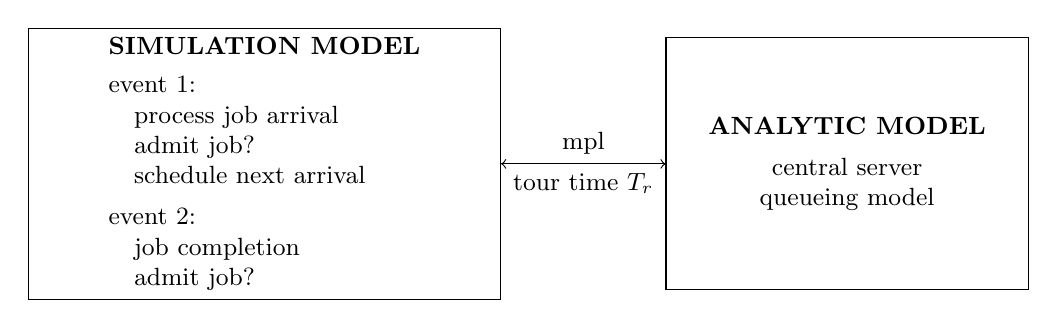
\begin{tikzpicture}[font=\small, line width=0.4pt]
  \node[draw, rectangle, minimum width=6.0cm, minimum height=3.2cm, align=left] (sim) at (-3.7,0)
  {\textbf{SIMULATION MODEL}\\[0.3em]
   event 1:\\
   \quad process job arrival\\
   \quad admit job?\\
   \quad schedule next arrival\\[0.4em]
   event 2:\\
   \quad job completion\\
   \quad admit job?};

  \node[draw, rectangle, minimum width=4.6cm, minimum height=3.2cm, align=center] (ana) at (3.7,0)
  {\textbf{ANALYTIC MODEL}\\[0.4em]
   central server\\
   queueing model};

  \draw[->] (sim.east) -- node[above] {mpl} (ana.west);
  \draw[->] (ana.west) -- node[below] {tour time $T_r$} (sim.east);
\end{tikzpicture}
\caption{Simulation and Analytic Components of the Hybrid Model}
\end{figure}

The simulation model generates arrivals, determines when a job is to be
admitted into execution, computes job completion times, schedules job
completions, and accumulates performance measurement data when jobs complete.
It computes the next job completion time by finding the job with the smallest
number of CPU-disk tours remaining, invokes the analytic model to determine
the mean tour time, and computes how long that number of tours will take. To
compute the mean tour time, the analytic model requires mean CPU and disk
service times, disk routing probabilities, and the number of jobs executing
(i.e., the multiprogramming level, or mpl). For simplicity, we'll assume that
mean service times and routing probabilities are the same for all jobs and are
established when the model is initialized. Consequently, the analytic model
only needs the current mpl to compute the mean tour time. Note that, if
desired, we could change the service times and routing probabilities of the set
of active jobs as jobs enter and complete execution.

The event routines and functions of the simulation model component are
outlined in Figure 3.3. arrival is caused when a job arrival event occurs. It
generates the attributes of the job, enters the job in the admission queue,
schedules arrival of the next job, and calls the job scheduling function to
determine if the job can be admitted to execution. One of the attributes
generated for a job is the number of CPU-disk tours to be executed.

The job scheduling function, job\_schedlr, is called whenever a job arrives or
leaves the system. It scans the admission queue for a job which satisfies the
rules of the admission policy. If such a job is found, update is called to
update tour counts (since placing another job in execution will change the mean
tour time). update calls the solve function to evaluate the analytic model and
compute the mean tour time. The time elapsed since the last update is divided
by the mean tour time to determine the mean number of tours completed since
then, and the tour counts of the active jobs are decremented by that number.
job\_schedlr then dequeues and activates the selected job and increments the
multiprogramming level. Increasing the number of jobs in execution will affect
tour times, making the scheduled next job completion event invalid, so it is
cancelled (it also is possible that the newly-activated job may complete
execution before any other job). The next\_completion function is called to
schedule the next completion. Although not shown in the outline of Figure 3.3,
the scheduling function should go on to try to activate additional jobs, since
completion of one job might free enough memory space to permit several jobs to
enter execution.

The next\_completion function scans the set of active jobs to find the one with
the smallest number of tours remaining. It invokes the analytic model to
determine the mean tour time, computes the remaining execution time for that
job by multiplying the number of tours by the mean tour time, and schedules
completion of that job.

The completion event routine is ``caused'' when a job completion event occurs.
It updates tour counts, deactivates the completed job (i.e., deallocates its
job descriptor table entry), and accumulates job performance measures, such as
the time spent in the system. It calls next\_completion to schedule the next job
completion, and calls the job scheduling function to see if jobs in the
admission queue can now be activated.

Job measures such as the mean system residence time and the mean number of
jobs in the system are computed using the methods described in Sections 1.4
and 1.5. Performance measures for entities of the analytic model are computed
by collecting measures for each inter-update interval and weighting them
 either by the relative interval length or relative number of operations in the
interval. (As a practical exercise in applying operational analysis, try
working out the computation of overall throughput, utilization, mean queue
length, and mean residence time for the CPU.)

\begin{figure}[ht]
\centering
\begingroup\small
\begin{verbatim}
arrival event routine
  generate job attributes:
    ... memory requirements
    ... no. of tours (Nt)
  job -> admission queue
  schedule next arrival
  call job_schedlr
  cause next event

job_schedlr function
  return if no job satisfies admission rules
  call update
  dequeue & activate selected job
  mpl += 1
  cancel currently-scheduled completion
  call next_completion
  return

update function
  call solve to compute mean tour time (Tr)
  compute mean no. of tours completed since last update (n)
  decrement tour counts (Nt) of all active jobs by n
  return

next_completion function
  find active job (job i) with smallest no. of tours
  call solve to compute mean tour time Tr
  schedule job i completion: te = Nt(i) * Tr
  return

completion event routine
  call update
  deactivate job, accumulate job performance measures
  mpl -= 1
  call next_completion
  call job_schedlr
  cause next event
\end{verbatim}
\endgroup
\caption{Hybrid Model Event Routines and Simulation Functions}
\end{figure}

Hybrid modeling can provide substantial savings in computation time. In our
example, there are only two events per job (ignoring cancelled events) and
only two events in the event list at any time, so the simulation part is very
fast. The analytic model has to be evaluated only on job activation and
completion. The number of arithmetic operations required for its exact
solution is proportional to the product of the multiprogramming level and the
number of servers, and this should be small compared with the number required
 to simulate a job's disk requests. Even faster solutions can be obtained using
approximation methods. Schwetman [1978] compared hybrid and simulation models
of several systems, and reported CPU time improvement factors ranging from 18
 to 200. The improvement for a particular model depends on the relative
complexity of the analytic model and the simulation model it replaces.

Hybrid modeling is not applicable in every situation. The analytic model
usually requires stronger assumptions than the simulation model it replaces,
and this won't always be acceptable. The hybrid model discussed here adds the
assumption that the use of mean, rather than actual, tour times does not
significantly affect job residence times. This assumption is based on the
notion of decomposability in the sense used by Courtois [1977] (alternatively,
see Courtois [1975]). However, when the main functions of some parts of a
model are to establish an operating point for or provide work to the key part
of the model, the assumptions associated with these supporting parts often are
less critical. In such cases, it may be possible to replace a set of
simulation operations by an analytic function.

Given, for example, an analytic function for the distribution of operation
times, we can use the distribution's inverse to generate random operation
times. Sometimes a set of operations can be represented by a graph model whose
parameters (execution times, branching probabilities) are determined by
simulation. Rather than explicitly simulating these operations and scheduling
each execution time, it may be possible to obtain the mean overall execution
time and variance using analytic reduction methods (see Beizer [1978] or
MacDougall [1975]). Depending on model assumptions, this mean can be used as
the operation time, or the mean and variance can be used to generate a sample
operation time from a distribution. Some beforehand experimentation is needed
to determine the distribution's form.

Hybrid modeling is not discussed in any of the referenced simulation texts,
and receives only limited notice in most performance evaluation texts. Most of
the useful reference material has appeared in the form of technical conference
and journal papers. Schwetman's work (cited earlier) provided much of the
impetus for current work in this area. Chiu and Chow [1978] describe its
application to a complex computer system model. Shanthikumar and Sargent
[1983] divide hybrid models into four classes, discuss each class, and give
several examples of hybrid modeling. Blum et al.\ [1984] present experimental
comparisons of hybrid, analytic, and simulation models, and discuss advantages
of and problems in decomposition. Thomasian and Gargeya [1984] describe a
two-phase procedure for modeling a memory-constrained timesharing system with
 two customer classes. In the first phase, an analytic model is used to compute
system throughputs for the possible combinations of customers; these
throughputs are input parameters for the second phase, which uses a
simulation model to estimate mean response times. O'Reilly and Hammond
[1984] describe an approach to local area network modeling in which some
stations in the network are represented individually via simulation while the
remaining stations are represented collectively by an analytic model. This is
not a complete list; other examples can be found by reviewing the technical
literature in your area.

\section{Simulation Program Development}
\label{sec:simulation-program-development}

Developing a simulation program is very much like any other program
development task, although the quasi-concurrent nature of simulation program
execution sometimes gives it an operating system flavor. The main
considerations are

\begin{itemize}
\item simulation model design
\item program organization
\item parameter management
\item debugging aids
\item instrumentation
\end{itemize}

We'll discuss the first three topics in this section; debugging and
instrumentation are discussed in later sections.

\paragraph{Simulation model design.}
After deciding upon simulation as the analysis method, the next step is to
transform the model description into a simulation model design. This is -- or
at least should be -- the first point in the modeling process at which the
simulation language's view is imposed on the model. Our language is
event-oriented, so the model design defines sequences of activities with their
initiating and terminating events. However, if the model is complex, we
should try to approximate a process-oriented view by developing separate
definitions for different classes of processes (where a process can be a job, a
 task, or a request). This essentially involves defining a separate
 event-oriented model for each class and specifying any inter-model
coordination required (in addition to that provided by facilities). In
designing this model, we should try to maintain as much resemblance between
it and the system design as is reasonable at the model's level of abstraction.
(This similitude of model and system doesn't guarantee model validity, but is a
great help in achieving it.) As we outline activity and event sequences, the
data used at each step is identified and data structures developed for each
process class. A manual simulation of the final design can help catch errors
of omission.

\paragraph{Program organization.}
The next transformation is from model design to program design. The
organization of the program depends on the complexity of the model. For
simple models with few activities, the simulation program may look much like
those of Figures 1.7 and 2.2 -- a single procedure with events identified by
number. For somewhat larger models, we'll probably use separate function
procedures for each event routine and define events symbolically for easier
program modification. For complex model designs, where we've defined separate
models for each class of process, the program is organized as a set of
submodels, each of which may comprise a set of function procedures. (There is
 a limit on how complex a model we should attempt using smpl or any other
event-oriented language.) Some submodels may be combined at this point
(perhaps just to reduce code volume) in which case their data structures have
to be merged and modified.

Organizing the simulation program as a set of submodels representing different
process classes is facilitated by smpl's implicit queueing. Individual
submodels can execute independently, performing any necessary coordination
via operations on facilities. Explicit queueing would require that submodels
operate directly on one another. In modeling process coordination mechanisms,
smpl facilities can be used to represent such diverse entities as a hardware
flip-flop controlling a buffering operation or an operating system semaphore.
This representation range is somewhat limited by the inability to dynamically
create and destroy facilities (although smpl could be extended to provide
this).

The events defined in the simulation model design may be split or may be
combined into simulation program event routines. An activity initiation event
may have to be split into two event routines when it involves facility
reservation, since a blocked facility request results in reexecution of the
event routine which issued the request. Statements which should not be
reexecuted, such as those selecting the facility to be reserved or the token
involved in the operation, should be placed in a separate event routine (for
the reasons discussed in Section 2.4).

When an event representing the end of one activity and an event representing
 the initiation of another activity occur at the same instant in simulation
time, some code and execution time can be saved by combining both events in
one event routine. There are several things to consider before doing this. If
the event routine contains a facility request, reexecution of the routine
following a blocked request will cause problems. When the two activities
belong to logically different classes and the events coincide simply because
one activity freed a resource needed by the other, the loss of structure
resulting from combining event routines may not be worth the slight gain in
efficiency. Even when the activities belong to the same class and are
logically connected, debugging and expandability considerations may make
separation of event routines worthwhile.

For complex models, a top-down iterative approach to simulation model
development and programming is recommended. In this approach, the model is
initially defined at a high level of abstraction, comprising a small number of
macroscopic activities, perhaps defined only in terms of their execution
times. The level of detail of the model and the program are advanced in a
series of steps. At each step, (only) one activity of the model is refined into
a more detailed representation, and the simulation program is revised,
debugged, and verified at this new level of detail. At any point in model
development, the simulation program is executable and verifiable; each advance
in the level of detail can be checked against the preceding level.

\paragraph{Parameter management.}
Assigning values to model parameters is one of the more tedious aspects of
simulation program development. We have to decide which parameters we want to
assign values to from outside the program (i.e., at run time) and which will
be assigned values within the program (at compile time). Usually we will
considerably under-estimate the number of parameters we'll want to vary at run
 time.

There is one commandment for specifying parameters within the program: don't
``hardwire'' numeric values in the code. If we do, we'll inevitably have to
change them and, with equal inevitability, we'll miss one. The C macro
facilities are very helpful in this regard, not only in defining simple
symbolic constants but also in doing things like switching random variate
sampling functions.

Simulation program size and use determine how much effort to expend in
developing capabilities for run time input of parameter values. A large number
of parameters, or program use by other than the developer, justify a certain
amount of sophistication in the way of an input language as well as some error
checking. The development effort required can be surprising. In some large
simulation programs, one-third of the code is input processing, one-third is
report generation, and a modest one-third represents the model itself.
However, even the smallest model is much more convenient to use if an input
processor is provided, and we might as well implement it at the start, rather
than waiting until we get tired of recompiling. SMPL provides facilities for
defining and labeling input and output parameters, assigning input parameter
values either from the simulation program or from a display, and reporting
output parameter values (see Chapter 7). These facilities, although simple,
have proved to be very useful.

Defining values of compile-time parameters and providing input facilities for
specifying values of run-time parameters doesn't completely solve the
parameter management problem; we also need to tabulate parameter values as
part of model output. If we don't, we'll frequently find ourselves staring at a
simulation report and wondering under what conditions the results were
obtained.

\section{Simulation Program Debugging}
\label{sec:simulation-program-debugging}

Debugging is the task of getting the simulation program to the point where we
think it works -- it runs without errors and the results it produces seem
reasonable. Verification is the task of proving, as best we can, that the
program is a valid implementation of the model.

The tools used in simulation program debugging are the traditional ones: error
diagnostics, traces, dumps, and reports, all blended with a judicious
sprinkling of print statements. smpl error messages, traces, and reports were
 described in Chapter 2. SMPL adds a dump capability which shows the contents
of the event list and queues, and the status and users of each facility. You
may want to add a similar capability to your version of smpl (an example
appears in Chapter 7).

For small models, the standard smpl debugging aids, perhaps supplemented by
user trace messages and print statements, usually are adequate. Large models
should have trace, dump, and other debugging aids designed into the program
from the start. These should provide a logical view of model operation. To
control the volume of output, they should provide selectable levels of detail
for selectable parts of the model. Particular attention should be given to
model data structures: errors often occur in the dynamic allocation and
deallocation of token attribute records, particularly in the management of
associated indexes and pointers.

The procedure outlined below has proven to be efficient in the early stages of
program debugging.

\begin{enumerate}
\item On the first successful compilation of the program, try executing it.
Maybe it will run the first time out; in any event, we need to get the notion
out of our system!

\item Set up the simulation program to execute a single token, turn tracing
on, and trace the execution of this token. Review the trace data and the
simulation report to determine if the program executed correctly. It should be
straightforward to locate any problems.

\item Now revise the setup to execute two tokens sequentially (so that
execution of the second token can't begin until execution of the first token
completes), and again trace and review token execution. The objective is to
find problems left behind by the first token, such as facilities that didn't
get released, data elements that didn't get deallocated, and so on. Printing
values of pointers and indexes can help identify problems.

\item Revise the program once again to execute two tokens concurrently, trace
token execution, and look for problems in the interaction of the two tokens.
It may be necessary to initiate execution of the two tokens at the same time
to insure that queueing, preemption, or other resource conflicts occur. Verify
the flow of each token from event to event: problems in event routine
organization, such as unplanned reexecution of statements, often show up as
breaks in this flow.

\item Expand on this controlled execution process if the model is complex. For
example, the program can be modified to direct tokens along specific execution
paths, or to examine limit conditions such as communication network node
blocking on a packet limit. Sometimes the process can be simplified by
isolating submodels (or simply sections of the model) and driving them
independently.

\item When selective execution no longer turns up errors, try full execution
of a modest number of tokens. Watch the trace awhile to see if queues build up
because facilities aren't getting released. If a simulation error occurs, note
the time of its occurrence. Add an event routine to the simulation program to
turn tracing on, and schedule this event to occur some time earlier than the
error. (With SMPL, this can be done by setting breakpoints from the keyboard.)
How much earlier is a matter of guesswork: cause and effect may be widely
separated in time. The errors initially found at this step frequently are
caused by ``end game'' problems: conditions reached for the first time in
program execution, such as allocation of the last element in a free element
list.

\item When the model runs to completion without errors, review the simulation
report. Look at utilizations, queue lengths, and distributions of requests
across facilities to see if the values make sense intuitively and if they are
consistent in an operational analysis sense. In some cases (e.g., more than
one token class), this analysis may require adding instrumentation on the
simulation program. If the results are operationally correct but
counter-intuitive, find out why: there may be an error in service time
computation or an unanticipated (but perhaps valid) delay situation.
\end{enumerate}

In the personal computer arena, several C tools are available which could be
used to advantage in simulation program debugging; these include debugging
environments and C language interpreters. Another tool which has been
occasionally useful in debugging is the SMPL time series display (see Chapter
6). This display can be used to plot facility utilization, instantaneous or
average queue length, or a specified parameter value, versus time. When things
go awry at some point during execution without an error being detected, the
effects sometimes can be seen in the queue length display.

\section{Verification}
\label{sec:verification}

When the program produces reasonable results, debugging can be considered
complete (at least until a parameter change or use of a different random
number stream turns up another error), and we can turn our attention to the
next problem: verifying that the simulation program is a valid implementation
of the model. For small models, this may be obvious from inspection; for larger
models, some substantiating analysis is needed.

At a minimum, verification requires a comparative ``walkthrough'' of the model
description and the simulation program. Sometimes this is all that is
feasible, and success of the analysis effort depends on how diligently it is
done. However, additional verification via comparison with analytic models
often is possible. The simulation program is modified to represent a model for
which analytic results can be obtained, and the simulation and analytic results
are compared. This analytic verification does not, of course, guarantee that
the program matches the model. However, it does provide a way to eliminate
errors in at least part of the modeling process. If analytic verification is
successful, then any remaining errors are either in transforming the model
description to a model design or extending assumptions from the analytic model
to the simulation model.

A careful review is the only means of verifying the transformation of model
description to model design; however, since analytic verification involves
both simulation and analytic model design, it provides some cross-checking.
The extensions from analytic model to simulation model (suppressed for
verification) may take various forms, including distributional assumptions,
added level of detail, queueing disciplines, and token classes and priorities.
Although it may not be possible to analytically verify these extensions in the
context of the complete model, it may be possible to isolate parts of the
model and verify them independently. Sometimes a subsection of a closed system
model can be verified by isolating it and treating it as an open system model,
adding the necessary event routines to generate arrivals and handle
departures. In any case, extensions should be informally checked as part of
the process of returning the simulation program to its original form. We'll
often have some idea of what the effect of a changed assumption should be, and
can at least check to see that results change as expected. For example, if we
changed a distribution from hyperexponential to exponential for purposes of
verification, we would usually expect to see queueing increase when the
distribution was restored to a hyperexponential one. If we isolated part of
the model and verified that part in an open system, we would expect its
queueing delays to decrease when it becomes part of a closed system with a
finite number of customers.

The work involved in analytic verification can be reduced substantially by
planning for it at the start -- providing parameters to control extensions,
and developing, debugging, and verifying the model hierarchically. The only
hazard in this is a tendency to bias model development toward verification,
rather than application.

Where do we find analytic models to use in verification? For a variety of
single-queue, single- and multi-server open queueing systems, closed-form
expressions for expected values of parameters such as mean queue length and
residence time can be found in several of the referenced texts, in particular,
Allen [1978] and Kleinrock [1975]. Less extensive coverage appears in Banks
and Carson [1984], Kobayashi [1978], and Trivedi [1982]. Both Allen and
Kobayashi present results for the simplest closed queueing system, the machine
repair model. A simple algorithm for solution of central server queueing
systems was devised by Buzen [1973]; these systems are discussed in Kobayashi,
Trivedi, and several other texts. Ferrari [1983] provides a comprehensive
discussion of Buzen's algorithm, including load-dependent servers, and
includes a Fortran implementation of a central server model for computer
system analysis. However, the central server model is just a particular form
of queueing network; algorithms for the solution of more general network forms
are available. Lazowska et al.\ [1984] provide Fortran programs for the
solution of single job class and multiple job class networks. These are useful
in their own right for the task we're considering here; using the techniques
and algorithms described by Lazowska et al., these programs can be tailored
and extended as required in a particular application environment, and are
useful in analysis as well as verification. Finally, in addition to general
analytic models, specific analytic models from the technical literature can be
useful in verification, particularly when they have been validated.

The results obtained from simulation rarely, if ever, will agree exactly with
those obtained analytically. Simulation is a sampling process; in a simulation
experiment, we generate a large number of sample values and use the sample
mean as an estimate of the actual mean. Consequently, some difference between
simulation and analytic results can result from sampling variation. If this
 difference is small, we may not worry about it. Alternatively, we can carry
the analysis further: collect additional data, compute confidence limits for
the simulation estimate, and determine if these limits include the analytic
result. (This output analysis process is discussed in the next chapter.) For
reasons discussed in the next section, we should not expect to see comparable
percentage differences for all measures.

Another possible source of variation between analytic and simulation results is
approximations used in the analytic model. If the analytic model is one we've
developed ourselves, we are at least aware that approximations are used, and we
may be able to ``back off'' to an exact solution. If we're using a queueing
analysis package of some kind, result variations can be hard to interpret.
Package solution methods and use of approximations often are considered
proprietary and are not documented. (However, problems usually arise only when
the package is used differently than intended.)

\section{Validation}
\label{sec:validation}

Validation is the task of demonstrating that the simulation model is a
reasonable representation of the actual system: it reproduces system behavior
with enough fidelity to satisfy analysis objectives. The question of how much
is enough can be answered only in terms of these objectives and perhaps the
results obtained in the current iteration of the analysis process. For
example, demonstrating that a model tracks real-system trends may be
sufficient in a comparative analysis in which one alternative significantly
outperforms the other. On the other hand, when a critical system parameter
must be estimated within a few percent, the simulation model must be
demonstrably capable of providing that accuracy. The simulation model usually
is developed to analyze a particular problem and may represent different parts
of the system at different levels of detail. The model doesn't have to be
equally valid for all parts of the system over the full spectrum of system
behavior; it just has to meet the requirements of the problem.

The subject of validation gets terse treatment in our simulation texts. Of
these, Banks and Carson [1984] provide the best coverage, followed by Law and
Kelton [1982]. The discussion and references in Sargent [1984] provide a good
starting point for reviewing the literature. Balci and Sargent [1982] provide
a bibliography indexed by validation technique and by the statistical
technique used to compare measurement data and model results. Schatzoff and
Tillman [1975] and Teorey [1975] describe validations of computer system
simulation models. Schatzoff and Tillman illustrate the use of experiment
design methods and probability plots in simulation model validation; Teorey
presents a procedure for validation and illustrates it by application to an IO
subsystem model.

For purposes of this discussion, there are two different cases of validation to
consider. In the first case, the system being modeled exists and can be
measured, the analysis objective is to evaluate a proposed change to the
system, and validation is based on comparison of model results with
measurements. In the second case, the system being modeled exists only as a
design, and the analysis objective is to estimate performance of the design or
perhaps to evaluate alternative designs; little or no comparative data exists,
and validation mostly is a matter of design-model comparison.

\paragraph{Validation of models of existing systems.}
In this case, measurements of the existing system are compared with results
from a simulation of the existing system; if they agree, it is assumed that a
simulation of the modified system will produce valid estimates of the effects
of the proposed change. It all sounds so simple! The only problems are
measurement, comparison, and extrapolation.

Collecting system performance measures for use in validation ideally is done
when collecting workload characterization data. Conceptually, we want to
collect workload data over some period of operation, collect system
performance measures over that same period, drive the simulation model with
the workload data, and compare model results with measurements. Practically,
this can be hard to do. Measurement tool limitations can make it difficult to
match workload and performance data: for example, work in execution at the
beginning and end of the measurement period may not be properly accounted
for, and lengthening the measurement period is not always a solution.
Available performance measures may be incomplete, inconsistent or overlapping,
and not at the desired level of detail.

A number of measurement problems can be avoided or at least identified in
advance by developing a measurement model of the system. The measurement
model is derived from the analysis model description. It defines the
measurements and measurement points required for a complete description of
system performance, in an operational analysis sense, at the desired level of
detail. While it may not be feasible to instrument the system to provide these
measures, this model provides a framework to evaluate and apply available
measurements. The objective is to try to match these measurements to those
defined in the measurement model, adjusting the measurement points defined in
the model and the level of detail of parts of the model if necessary but
maintaining completeness if at all possible. (The difficulties in doing this
emphasize the need for something better than the usual ad hoc approach to the
design of system measurement facilities.) The final version of the measurement
model itself is validated by comparing aggregated workload data with traffic
and utilization measures.

Once the measurement model has been developed, the simulation model's
instrumentation should be revised or extended to report the same performance
measures as the system. Measures can be reported in the form of means, means
and variances, or distributions. While we can instrument the simulation model
 to provide any form, system measurement facilities often limit the forms in
which measurement data can be reported. Because of both reporting limitations
and statistical considerations, comparison of measurements and model results
generally is based on mean values.

The only test we can apply to a comparison of mean values from one measurement
period with means from one simulation run is a subjective one: how close are
the values? Except for trace-driven models, the work performed by the
simulated system and by the actual system are the same only in a statistical
sense; differences in measurement and model values arise because of sampling
variation as well as because of simplifying assumptions made in modeling. In a
subjective comparison, we rely on our judgement to determine if the values are
``close enough.''

In making this comparison, we shouldn't expect the same percentage difference
for all measures. To see why, consider an M/M/1 queueing system. The mean
number of customers in this system can be defined in terms of server
utilization as follows:

\begin{equation}
L = \frac{U}{1-U}
\end{equation}

The percentage change in $L$, $P_L$, resulting from a percentage change of
$P_U$ in $U$ can be obtained via differentiation:

\begin{equation}
P_L = \frac{P_U}{1-U}
\end{equation}

For example, at a base utilization of 0.5, a five percent change in
utilization translates into a ten percent change in the mean number in the
system. Consequently, a difference in measurement and model facility
utilizations can result in a larger difference in measures such as queue
length and response time, independent of all other effects. The magnifying
factor of the second equation applies only to the M/M/1 queueing system. It
will be smaller for some systems (e.g., systems with limited population or
lower service time variance) and larger for other systems; in most practical
cases it won't be explicitly known.

Other subjective validation methods include comparison of distributions. If
measurement facilities permit reporting the distribution of values of, for
example, system residence time, we can instrument the model to produce a
corresponding distribution, and compare -- by inspection -- the two
distributions. (A statistical comparison is not possible because the sample
values forming these distributions are not independent.) If the tails seem
significantly different, remember that they may represent only a few sample
values. The SMPL table facility (see Chapter 9) can be used to collect,
tabulate, and plot distributions of simulation data; it can also be adapted for
use in post-measurement data reduction.

Statistical techniques for comparing measurement and simulation results are
discussed in the references cited earlier in this section. In the simplest
case, multiple simulation runs are made to obtain the sample mean and sample
standard deviation for the simulation value, and a $t$ test used to decide if
the results are ``close enough.'' This is easy to do and we often want to
compute confidence intervals for simulation results anyway, as we'll discuss in
 the next chapter. In other cases, multiple sets of measurements are required,
and the additional data collection effort can pose problems unless planned in
advance.

We'd like to validate the model over a range of operating conditions broad
enough to encompass the planned analysis. (Doubling the validation points from
one to two will much more than double our confidence!) However, doing this --
particularly collecting the required measurement data -- can be costly. A
formal method for analyzing experimental cost versus the risk of accepting an
invalid model has been proposed by Balci and Sargent [1981], [1982]. While the
method may be outside the scope of the studies envisioned here, the discussion
of validation hypotheses is worth reviewing.

When the difference between measurements and simulation results is more than
we're willing to accept (or able to rationalize), we face a chore called
(euphemistically) model calibration. At some point in the modeling process, we
made a mistake. Most often it will be one of omission and will result in model
values being less than measured values. The problem may be an invalid
simplifying assumption. This assumption may have been made implicitly, so --
 in addition to checking explicit model assumptions against the system -- we
need to review system operation to see if we've left something out. Close
comparison of measurement and model data may provide some clues, as when queue
lengths agree in one part of the system but not another; this can result in a
quest for additional measurement data. Sometimes the problem is in data
collection: for example, operating systems often provide inadequate and
incomplete measurements of overhead time. In this case, the modeler is faced
with the temptation to ``calibrate'' (diddle) the model by adjusting model
input parameters to obtain output values which match the measurement data. (It
is hard to throw the first stone here.) Trying to find out why measurements and
model results don't agree can be very frustrating. It also can be very
rewarding, because it frequently provides new insights into system behavior.

When the model has been accepted as a valid representation, it is revised --
very carefully -- to represent the proposed change, and a new set of
simulation results are obtained and compared with those for the existing
system. Typically, the revised model uses the same set of workload parameters
as the validated model; we assume that the workload is unaffected by the
change. This assumption warrants examination: all systems are closed systems
with feedback effects if we look far enough. Although we may have only been
able to validate the original model at one or two points, we often want to
compare outputs of the original and revised models over a range of input
parameter values. Our confidence in the validity of analysis results depends
on the extent of the difference between the original and revised systems, and
will be higher for results obtained close to the validation points.

\paragraph{Validation of models of designs.}
When the system being modeled does not exist, validation primarily is done by
review; the model is examined in terms of the system design, and each
assumption and abstraction scrutinized and justified. This needs the
involvement of other design team members as reviewers, critics, and
contrarians; satisfying an expert audience is the best test of the validity of
model design and of system timing value assumptions. Workload parameter values
usually are determined by extrapolation from past systems. The design team's
review of these usually is based on judgement and experience, rather than on
the factual knowledge used to compare model and system designs: it may be
helpful to augment their review with one by knowledgeable system users.
Workload representativeness always is a concern; when the objective of the
analysis is an absolute prediction of the performance of the design, it is a
 key concern. When the objective of the analysis is a relative comparison of
design alternatives, we may be able to satisfy it using workload parameters
which are ``reasonable'', although not necessarily representative (see the
discussion in Section 3.4).

Similitude between system design and model is a key factor in validation. The
more the model resembles the design, the more likely is it to be valid, and
the easier it is for the reviewing designer to understand how the model
represents the design. Similitude is one aspect of what our simulation texts
refer to as ``face validity''. Correspondence of the simulation model to the
system design is guaranteed by a synthesis of design specification and
simulation model: ``the simulation is the design'' (Randell 1968). Simulation/
design synthesis is outside our scope: see MacDougall [1975] for a brief
discussion and additional references.

The two cases of validation described here represent ends of a spectrum. A
major change to an existing system presents much the same problem as a new
system design. Our confidence in a model of a new design is increased if we
can at least validate the approach with a similar model of an existing system.
In practice, validation often is blended with verification. If comparison of
measurements and model results is successful, then the simulation program is
assumed to be both a valid implementation of the model design and a valid
representation of the system. In modeling a new design, comparisons of
simulation program versus model design and of model design versus system
design tend to be done concurrently.

The final step in validation takes place when the system change is made or the
system design implemented, and predicted and actual performance can be
compared. This, unfortunately, doesn't happen very often in practice. The
final implementation may differ from the original design for reasons not
related to performance, and, in any case, the modeler is busy with a new
project and has little interest in auditing old work. In a system design
environment, there seldom is much pressure to carry out validation studies;
once the analysis has been done and the design decision made, alternatives are
discarded and the system gets built. The model becomes of historical interest
only, so few modelers ever pay for their sins. However, you will never know
how good or bad your analysis was unless you validate its results by
comparison with system measurements.

\section{Problems}
\label{sec:model-development-problems}

\begin{enumerate}
\item Estimating performance bounds sometimes eliminates the need for more
elaborate analysis and, in any case, provides a way of determining that our
simulation results are at least sensible. For a timesharing system such as that
of problem 3, Chapter 2, Lazowska et al.\ [1984] give asymptotic bounds for
throughput and response time.\footnote{Another method of bounds analysis called
balanced system bounds was developed by Zahorjan et al.\ [1982], and is
discussed by Lazowska et al.\ Balanced system bounds are ``tighter'' than
asymptotic bounds, and so are more useful for checking simulation results. The
discussion of bounds analysis in Chapter 5 of Lazowska et al.\ is recommended
reading.} The validity of these bounds depends only on the assumption that the
service time of one terminal request does not depend on the number or location
of other requests.

Let $D_k$ be the mean service demand (time) of a terminal request at server
$k$. Define $D = \sum D_k$ as the sum of the service demands of a request for
all $K$ servers, and define $D_{\max} = \max(D_1, D_2, \ldots, D_K)$ as the
largest service demand for any server. $X$, $R$, and $Z$ denote the
throughput, response time, and think time.

Consider throughput first. With a single terminal, there are no delays and the
throughput is $1/(D+Z)$. With $N$ terminals, the throughput is at best
$N/(D+Z)$, assuming no request ever has to wait for another request. At worst,
 each request finds $N-1$ requests ahead of it, and incurs a delay of
$(N-1)D$, and the throughput is $N/(ND+Z)$. Since a (single) server cannot
have a utilization of greater than 1, throughput is limited by the server with
the largest service demand to $1/D_{\max}$. The resulting bounds on $X$ are
shown in Figure 3.4(a).

The response time for a system with a single terminal is $D$. In the best
case, no request ever is delayed by another, and the response time continues
equal to $D$ as $N$ increases up to the point at which the utilization of the
busiest server reaches 1. At this point and beyond, the throughput is limited
 to $1/D_{\max}$ and, by the Response Time Law, the response time from this
point on is $N D_{\max} - Z$. In the worst case, each request has to wait a
 time $(N-1)D$ for other requests and so has a response time of $ND$. Figure
3.4(b) shows the bounds on $R$.

\begin{figure}[ht]
\centering
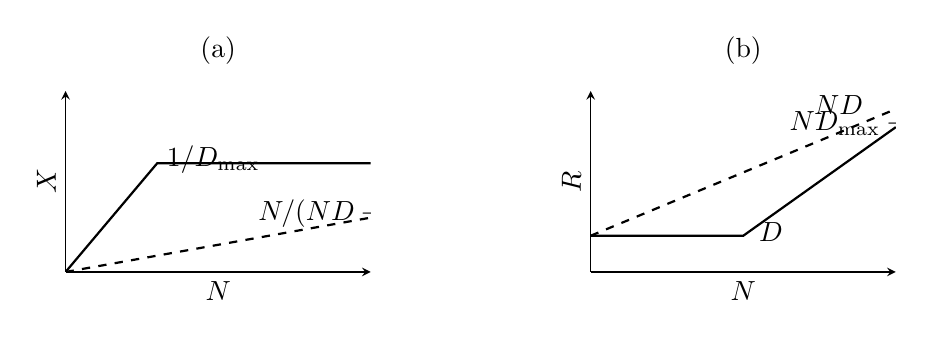
\begin{tikzpicture}
\begin{axis}[
  width=0.45\textwidth,
  height=0.32\textwidth,
  xlabel={$N$},
  ylabel={$X$},
  title={(a)},
  axis lines=left,
  xmin=0,
  ymin=0,
  xmax=10,
  ymax=1,
  ticks=none
]
  \addplot[thick] coordinates {(0,0) (3,0.6) (10,0.6)};
  \addplot[thick,dashed] coordinates {(0,0) (10,0.3)};
  \node[anchor=west] at (axis cs:3,0.62) {$1/D_{\max}$};
  \node[anchor=west] at (axis cs:6,0.32) {$N/(ND+Z)$};
\end{axis}
\begin{axis}[
  at={(0.55\textwidth,0)},
  anchor=origin,
  width=0.45\textwidth,
  height=0.32\textwidth,
  xlabel={$N$},
  ylabel={$R$},
  title={(b)},
  axis lines=left,
  xmin=0,
  ymin=0,
  xmax=10,
  ymax=10,
  ticks=none
]
  \addplot[thick] coordinates {(0,2) (5,2) (10,8)};
  \addplot[thick,dashed] coordinates {(0,2) (10,9)};
  \node[anchor=west] at (axis cs:5.2,2.2) {$D$};
  \node[anchor=west] at (axis cs:6.2,8.2) {$ND_{\max}-Z$};
  \node[anchor=west] at (axis cs:7,9.2) {$ND$};
\end{axis}
\end{tikzpicture}
\caption{Asymptotic Bounds for a Timesharing System (schematic)}
\end{figure}

Plot the throughput and response time bounds for the timesharing model of
problem 3, Chapter 2 for $N$ in the range 1 to 24. Locate the throughput and
response time values obtained from simulation on this plot. Assume that the
CPU in this system is replaced by a CPU of twice the speed, and plot response
 time bounds again.

\item The bounds described above can be applied to a ``batch'' system such as
that of Figure 2.1 by setting $Z$ to 0. Assume that, for any $N$, the
proportion of class 0 and class 1 tasks is the same as that in the model of
Figure 2.3. The CPU time per tour is the weighted sum of the class 0 and class
1 CPU times. The per tour service demand for a given disk is the product of
the visit ratio for that disk and the mean service time of that disk. The visit
ratio is the number of requests for that disk divided by the number of
requests for all disks, measured over an arbitrary interval. In this case,
visit ratios and service times are the same for all disks. Compute bounds for
the throughput (in tours per unit time) and mean tour time of this system.

\item An important verification technique (Section 3.9) is cross-checking
simulation and analytic model results, so queueing network analysis programs
are useful tools of the simulation modeler. While the analysis of networks
which involve such things as priority scheduling and simultaneous resource
possession (Section 5.5) may be relatively complex, some networks can be
analyzed using very simple programs. For example, Figure 3.5 shows a program
which can be used to analyze simple closed queueing networks with a single
customer class and in which all facilities -- service centers -- have single
servers with first-in, first-out queueing. The analysis method used by this
program is called exact Mean Value Analysis (MVA); for details and references,
see Chapter 6 in Lazowska et al.\ [1984].

\begin{figure}[ht]
\centering
\begingroup\small
\begin{verbatim}
#include <stdio.h>

#define real double

#define mxK 9 /* max. no. of service centers + 1 */
real D[mxK], /* D[k] = service demand at center k */
     R[mxK], /* R[k] = residence time at center k */
     Q[mxK], /* Q[k] = no. customers at center k */
     Z;      /* think time (0 for batch system) */
int K,       /* no. of centers (excl. terminals) */
    N;       /* no. terminals (mpl for batch) */

main()
{
    K = 3; N = 16; Z = 5000.0;
    D[1] = 12 * 40.0; D[2] = D[3] = 6 * (22.0 + 8.33 + 0.52);
    mva();
}

/* -- Exact MVA for Single Class, FIFO Center Networks -- */
mva()
{
    int k, n; real s, X;
    for (k = 1; k <= K; k++) Q[k] = 0.0;
    for (n = 1; n <= N; n++) {
        for (k = 1; k <= K; k++) R[k] = D[k] * (1.0 + Q[k]);
        s = 0; for (k = 1; k <= K; k++) s += R[k];
        X = (real)n / s;
        for (k = 1; k <= K; k++) Q[k] = X * R[k];
    }
    printf(" k    Rk     Qk     Uk\n");
    for (k = 1; k <= K; k++)
        printf("%2d%9.3f%7.3f%7.3f\n", k, R[k], Q[k], X * D[k]);
    printf("\nX = %7.4f, R = %9.3f\n", X, (real)N / X - Z);
}
\end{verbatim}
\endgroup
\caption{Queueing Network Analysis Program}
\end{figure}

This program can be used to analyze timesharing system models like that of
problem 3, Chapter 2, or batch system models like that of Figure 2.2 (although
only one job class can be represented). Inputs to the program are the number
of service centers $K$, the number of terminals $N$, the terminal think time
$Z$, and the demand at each service center $D[k]$. For a timesharing model,
$D[k]$ is the total service demand at center $k$ per terminal request. For a
batch model, $N$ is the multiprogramming level, $Z$ is 0, and $D[k]$ is the
average service demand at center $k$ per tour or per task completion,
depending on what unit we want to use in computing throughput and response
time. In Figure 3.5, main() sets parameter values for the timesharing model of
problem 3, Chapter 2. Note that main() specifies only the total service demand
per request; the number of CPU and disk operations per request is not needed
by mva(). The mva() function computes and tabulates, for each service center,
the mean residence time, mean queue length (which includes the customer in
service), and utilization. It also prints the system throughput and response
time.

Use this program to compute the throughput and response time of the
 timesharing system of problem 3, Chapter 2, for from 1 to 24 terminals. Plot
these values on the throughput and response time bounds plots of problem 1.
Change your simulation model of this system to use negative exponential disk
service times (with the same mean service time as the original model), and run
 the simulation with 2, 4, 8, 16, and 24 terminals. Mark the throughput and
response time values from these runs on your plots. Do the results tend to
verify your simulation model? For the 16-terminal system, how close are the
simulation results produced with exponential disk service times to those of
the original simulation?

\item Use the program of Figure 3.5 to analyze the queueing network model of
Figure 2.1. Compute the mean CPU queue length (including the task in service)
and mean CPU residence time from the simulation report of Figure 2.4. Compute
the relative difference in queue length and residence time between the
simulation results and the MVA results. How would you revise the simulation
model to obtain a ``tighter'' verification?

\item The program of Figure 3.5 can be used as the analytic component of a
hybrid model. Use this program to build a hybrid model of the timesharing
system of problem 4, Chapter 2, in which memory is represented simply by a
fixed multiprogramming level. Compare the results from the hybrid model with
those produced by the simulation model, and compare the execution times of
the two programs. Describe how you would extend this model to represent a
system with variable-length memory demands and allocation.

\item Develop a debugging and verification plan for the timesharing system
model of problem 6(b), Chapter 2, and carry it out. List the errors you find
(if any), and describe how they could be avoided in future models.
\end{enumerate}
